\documentclass[11pt,twocolumn]{article}
\usepackage{preamble}

\lhead{AST3310}
\chead{Term project 2: Modelling a Stellar Core}
\rhead{Bendik Samseth}
\lfoot{}
\cfoot{}
\rfoot{\fancyplain{}{\thepage}}

\title{Term project 2: Modelling a Stellar Core}
\author{Bendik \textsc{Samseth}}
\date{\today}
\begin{document}

\twocolumn[
\begin{@twocolumnfalse}
  \maketitle
  \begin{abstract}

In this report, this, that and more of this is discussed. All source
material related to this report can be found at the projects GitHub
repository~\cite{github}.    

  \end{abstract}
\end{@twocolumnfalse}
]

\section{Introduction}
When trying to understand the mechanics of a star, the most logical
place to start is with what we can observe. Let's take a look at the
properties of a star that we can measure with relative ease. 

Firstly, we can look at how much radiation energy hits one particular
area, i.e. a solar panel on earth. By assuming that the star radiates
equally in all directions we can calculate the total amount of energy
sent out by the star, the so-called luminosity (denoted as $L$).

In addition, we can find the surface temperature (denoted $T$) by
looking at the color of the light emitted from the star and using
Wien's displacements law. 

Lastly, we might be able to look at the orbits of all the planets and
do some number crunching and figure out the total mass of the star
(denoted $M$). This last part may be easier said than done, for
instance in the case of a far away solar system where we can't even
see the planets orbiting, just their minuscule effect on the stars
orbit. However, for the purposes of this report, let's assume that we
are able to do so. 

But that's about it for what we can figure out by just looking at the
outside effects. There are many other properties we would like to know
about, e.g. the radius ($R$), density ($\rho$) and pressure ($P$) of
the star. In particular, we would like to have all of these properties
as a function of the radius, so that we can get an idea of what the
cross section of the star looks like. In order to achieve this, we
need to deploy many different branches of physics, including
thermodynamics, hydrostatics and nuclear physics. And of course, a good
number of assumptions to simplify things for us.


\section{The Governing Equations}
In this project, we will only be looking at the radiative core of the
star. This means that we will not look at the outer convection layer,
and assume that all energy transport is done through photon
radiation. For reference, this corresponds to the inner $\sim 70\,\%$ of the
sun. Furthermore, we will not consider time evolution; we look at one
particular moment in time. 

The following four differential equations govern the internal
structure of radiative core of our star\footnote{Derivations of the
  equations are not given, as they are shown in the lecture
  notes~\cite{lecture-notes}. A qualitative description of their
  meaning is given instead.}:

\begin{align}
  \pd{r}{m} &= \frac{ 1 }{ 4\pi r^2\rho }\label{eq:drdm}\\
  \pd{P}{m} &= - \frac{ Gm }{ 4\pi r^4 }\label{eq:dPdm}\\
  \pd{L}{m} &= \epsilon\label{eq:dLdm}\\
  \pd{T}{m} &= - \frac{ 3\kappa L }{ 256 \pi^2 \sigma r^4T^3 }\label{eq:dTdm}
\end{align}

The first thing to notice about these equations are that they are
differentials with respect to mass, and not radius. Remember that what
we want in the end is all the properties of the star as a function of
radius, so it would make sense to write the equations with respect to
$r$ instead\footnote{I will use lower case $r$ and $m$ when referring
  to the radius and mass as variables, and upper case $R$ and $M$ for
  the total radius and mass.}. It turns out that it is more numerically
stable to use $dm$ compared to $dr$, so we are going to treat the
radius as $r=r(m)$. When we plot the data later, however, we will
return to using $r$ as the variable. Eq. \eqref{eq:drdm} is simply
stating the relation between taking an infinitesimal step in $r$,
compared to an infinitesimal step in $m$. 

Eq. \eqref{eq:dPdm} is the assumption of hydrostatic equilibrium, and
states that if the gas in the star is to be at rest, then the outward
pressure must exactly balance the force of gravity acting on the gas. 

The $\epsilon$ in Eq. \eqref{eq:dLdm} represents the amount of
energy produced by nuclear fusion per time and mass. This quantity
will be treated more in a later section (ref??).

Eq. \eqref{eq:dTdm} is the temperature gradient need to transport all
the produced energy out of the star. I should be noted that this is
only the correct temperature gradient when all the energy is
transported by radiation. 

\subsection{Equation of State}
In the equations~(\ref{eq:drdm}-\ref{eq:dTdm}) we use $T, \rho$ and
$P$. If we take a look at how many unknowns we have, we find that we
need one more equation. To this end, we are going to assume that we
can treat the gas in the star as an ideal gas, thus getting an
equation for the gas pressure through the ideal gas law:

\begin{align*}
  P_gV &= Nk_BT\\
  \Rightarrow P_g &= \frac{ N }{ V }k_BT = \frac{ \rho }{ \mu\,m_u }\label{eq:Pg}\numberthis,
\end{align*}
where $P_g$ is the gas pressure, $V$ is the volume, $N$ is the number
of particles and $T$ is the temperature of the gas.
The quantity $\mu\,m_u$ is the average mass of all particles in the
gas. $m_u$ is just a constant giving the average mass of a
nucleon. $\mu$ is slightly more complicated, and represents the mass
of the average particle in units of $m_u$ ($\mu$ is unit less). It
can be calculated a couple of ways. From the above equation we have

\begin{align}
  \mu &= \frac{\rho}{m_u}\frac{V }{ N } = \frac{ \rho }{ m_un_\text{tot} }
\end{align}
where $n_\text{tot}$ is the total number density of particles in the
gas. $n_\text{tot}$ can be taken as the sum of $n_i$ for all particles
$i$,

\begin{align}
  n_\text{tot} &= \sum_i n_i = n_e\sum_i \frac{ X_i\rho }{ C_i m_u}
\end{align}
where $X_i$ and $C_i$ is the mass fraction, and number of core
elements of particle $i$, respectively. For instance, $^4_2\text{He}$
gives $n_{^4_2\text{He}} = Y\rho/4m_u$, when $Y$ is the mass fraction
of Helium with four nucleons. The number density of the
electron, $n_e$ is written separate and should only consider the
number of \emph{free} electrons in the gas. In the case of only fully
ionized $^4_2\text{He}$, $n_e = 2n_{^4_2\text{He}}$ because each
ionized Helium core gives two electrons. I similar consideration
should be taken for each species present in the gas. 

Calculating $n_\text{tot}$ is not necessarily so straight forward, but
if we combine all the steps we have to take to compute $\mu$, we can
end up with a convenient formula:

\begin{align}
  \mu = \frac{1}{\sum (\text{particles provided per
  nucleus}\times\text{mass fraction}/\text{nucleons in core})}\label{eq:mu_0}.
\end{align}

This is the method used in the code, as a framework for summing over
all particles is central to the structure of the code base.


Let's now return to the original problem of finding an extra
equation. Eq. \eqref{eq:Pg} gives us an additional equation, but it
also introduces a new parameter, $P_g$. In addition to the gas
pressure, we have radiation pressure $P_{\text{rad}}$, so that the
total pressure is $P = P_g + P_\text{rad}$. Luckily, the expression
for radiation pressure is quite simple, and depends only on
temperature,
\begin{align}
  P_\text{rad} = \frac{ a }{ 3 }T^4
\end{align}
where $a = 4\sigma/c$ is a constant. This gives us finally the
additional equation of state we need;

\begin{align}
  P &= \frac{ \rho }{ \mu\,m_u }k_B T + \frac{ a }{ 3 }T^4\label{eq:P-eq_state}\\
  \Leftrightarrow \rho &= (P - \frac{a}{3}T^4) \frac{ \mu\,m_u }{ k_BT }\label{eq:rho-eq_state}.
\end{align}

I have listed the equation with respect to density as well; this
relation will be used to find $P$ given $\rho$ and $T$, and vice
versa.


\subsection{Energy Production}
In Eq. \eqref{eq:dLdm}, the quantity $\epsilon$ represents the amount
of energy produced per time and mass. We derive the value of
$\epsilon$ by looking at the reactions that produce energy inside a
star. It is given by
\begin{align}
  \epsilon = \sum_{ij}r_{ij}Q_{ij},
\end{align}
where $r_{ij}$ is the reaction rate for particles $i$ and $j$ (per
time and mass), and $Q_{ij}$ is the energy produced for each such
reaction. The exact values of $Q_{ij}$ can be found in the lecture
notes~\cite{lecture-notes}. More interesting is the rates, which are
given as

\begin{align}
  r_{ij} = \frac{n_in_j}{\rho(1+\delta_{ij})}\lambda_{ij}
\end{align}
where the symbols have their normal meaning (including the Kronecker
delta $\delta_{ij}$). $\lambda_{ij}$ is a complicated function of
temperature, and we will use tabulated expressions for these
functions, found once again in the lecture notes~\cite[Table
3.1]{lecture-notes}. 


There are a few different ways that fusion can happen, depending
on the conditions of the star. I our case we will simplify things a
bit and only consider the PPI and PPII chains (Proton-Proton based
fusion). 

One important thing to mention when calculating $\epsilon$ is that no
reaction should happen more often (have larger value for $r_{ij}$)
than the reaction(s) that produced the reactant(s) of the first
reaction. 

The last assumption we add is that all Deuterium produced by
Proton-Proton fusion, immediately fuses to $^3_2\text{He}$, thus
effectively merging the two first steps in the PP chains into one
reaction.


\section{Assumptions}
Up until this point, we've made several assumptions. In order to
remember the limitations of our results, I have summarized them in a
list:

\begin{itemize}
  \item Assume something.
\end{itemize}


\section{Solving the Equations}
At this point we are ready to start solving the governing
equations. For simplicity, I have chosen to deploy the standard
Forward Euler method. One should then note that the simplicity comes
at the cost of an global error proportional to the step size, $dm$. We
will try to be smart about this step size in order to minimize the
effects of this. 

As a reminder, Forward Euler solves a differential equation $du/dx =
f(u,x)$ by 
\begin{align*}
  u_{i+i} = u_i + du = u_i + f(u_i,x_i)\,dx.
\end{align*}

In our case, with four differential equations, this corresponds to the
following:
\begin{align*}
  r_{i+1} &= r_i +  \frac{ 1 }{ 4\pi r^2\rho }\,dm\\
  P_{i+1} &= P_{i} - \frac{ Gm }{ 4\pi r^4 }\,dm\\
  L_{i+1} &= L_i + \epsilon\,dm\\
  T_{i+1} &= T_i - \frac{ 3\kappa L }{ 256 \pi^2 \sigma r^4T^3 }\,dm
\end{align*}

\subsection{Choosing a Suitable Step Size $dm$}
When ever a numerical solution to a differential equation is tried,
one has to think about what step size $dm$ is suitable. In a perfect
world, we would like to set it to an infinitesimal number, but the
constraints of reality forces us to make a compromise between accuracy
and speed. We need to find a value for $dm$ that gives an accurate
enough result, but does so in a reasonable time. 

In order to evaluate the effect of different step sizes, figure
\ref{fig:dm-variation-no-dss} shows $r(m)$ calculated for a number of
different values of $dm$. From the figure we can see a large variation
in $r(m)$ for the lower values of $dm$. The solution seems to converge
when $dm \geq M_0\e{-3}$, but even there it is not perfectly
aligned. It turns out that the code runs very fast anyway (in large
part because it is written in C++), so it is no problem to crank the
step size down to $dm= M_0\e{-5}$, and still have do so in under a
second. 

\begin{figure*}[ht]
  \centering
  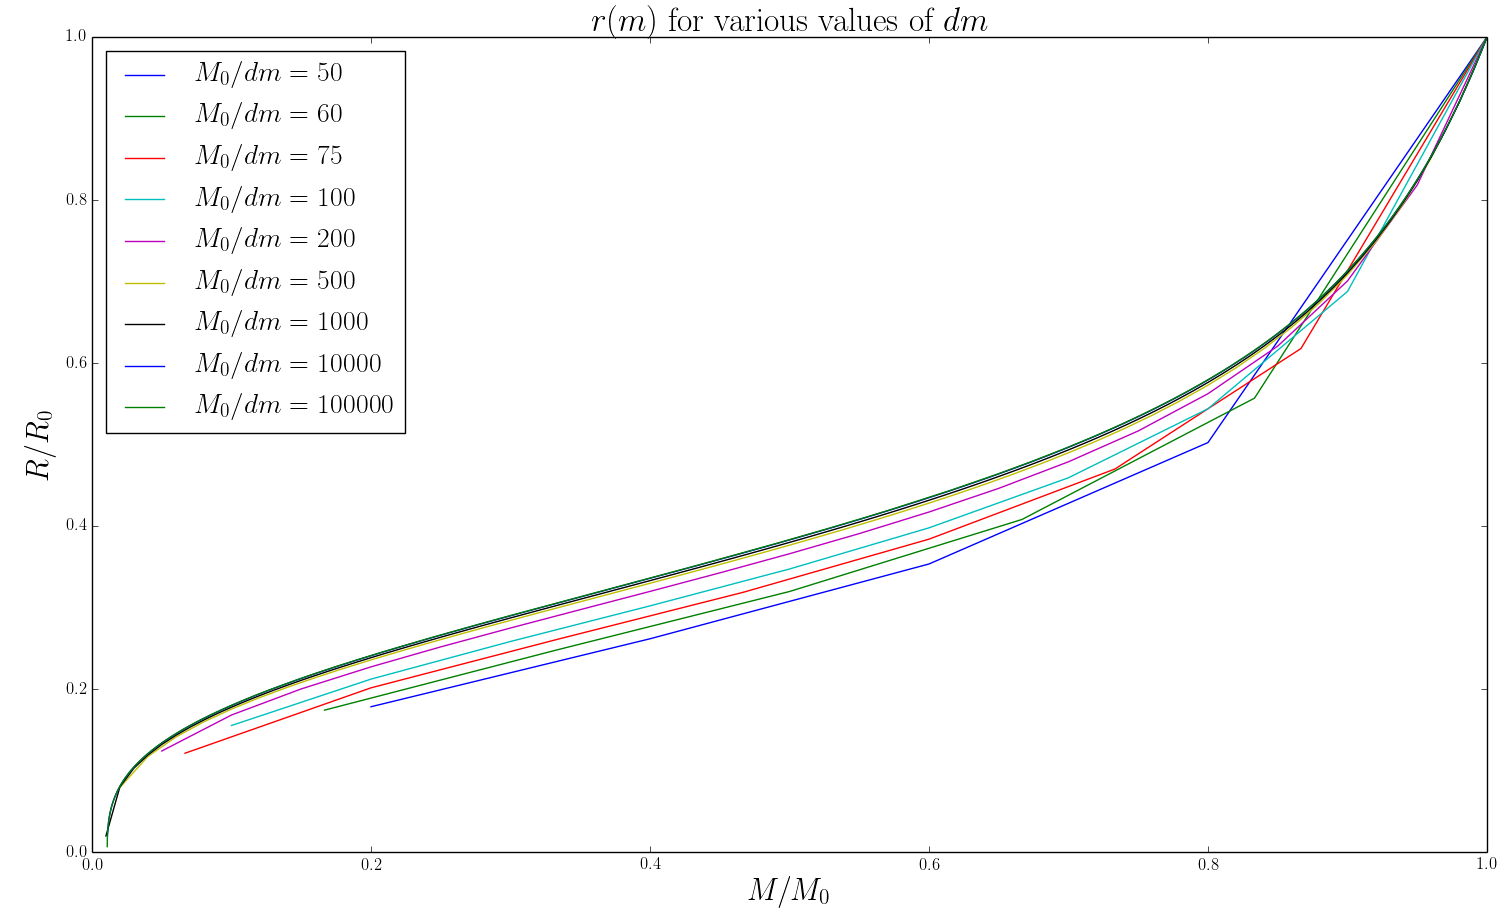
\includegraphics[width=\linewidth]{fig/dm_variation_no_dss.png}
  \caption{\label{fig:dm-variation-no-dss} Plots of $r(m)$ using a
    range of different values for $dm$. We see that we need quite a
    large number of steps in order for the solution to converge.}
\end{figure*}


This is quite neat, but we could still try to be a bit smarter about
this than just using brute force. The downside to setting a fixed value for $dm$ is that we might spend
a lot of computational time on a part of our function(s) that is very
stable, and on the other side, we might not have enough precision for
where the function(s) is very steep. The alternative is \emph{dynamic
  step size}, which involves defining the step size in such a way so
that the value of the function(s) does not change by more than a fixed
percentage. In the case of a diff.eq. $du/dx = f(u,x)$, we define the
step size in the following way:

\begin{align}
  \frac{du}{u} &\leq p\Leftrightarrow \frac{f\,dx}{u} \leq p\\
  \Rightarrow dx &= \frac{pu}{f},
\end{align}
where $p$ is the fraction that the solution is allowed to change by
after one step. In our case we have more than one equation, so we
impose a similar requirement to all equations and then simply choose
the smallest required step size.

The only thing we then have to define is what the value of $p$ should
be. As previously stated, the code is quite fast so we can afford to
be quite strict. The code used in all subsequent figures is set to
allow a maximum change of $1 \permil$. Figure \ref{fig:dm_variation}
shows the same plot as figure \ref{fig:dm-variation-no-dss}, but this
time including dynamic step size as well. The figure shows that DSS
gives good results. 

\begin{figure*}[ht]
  \centering
  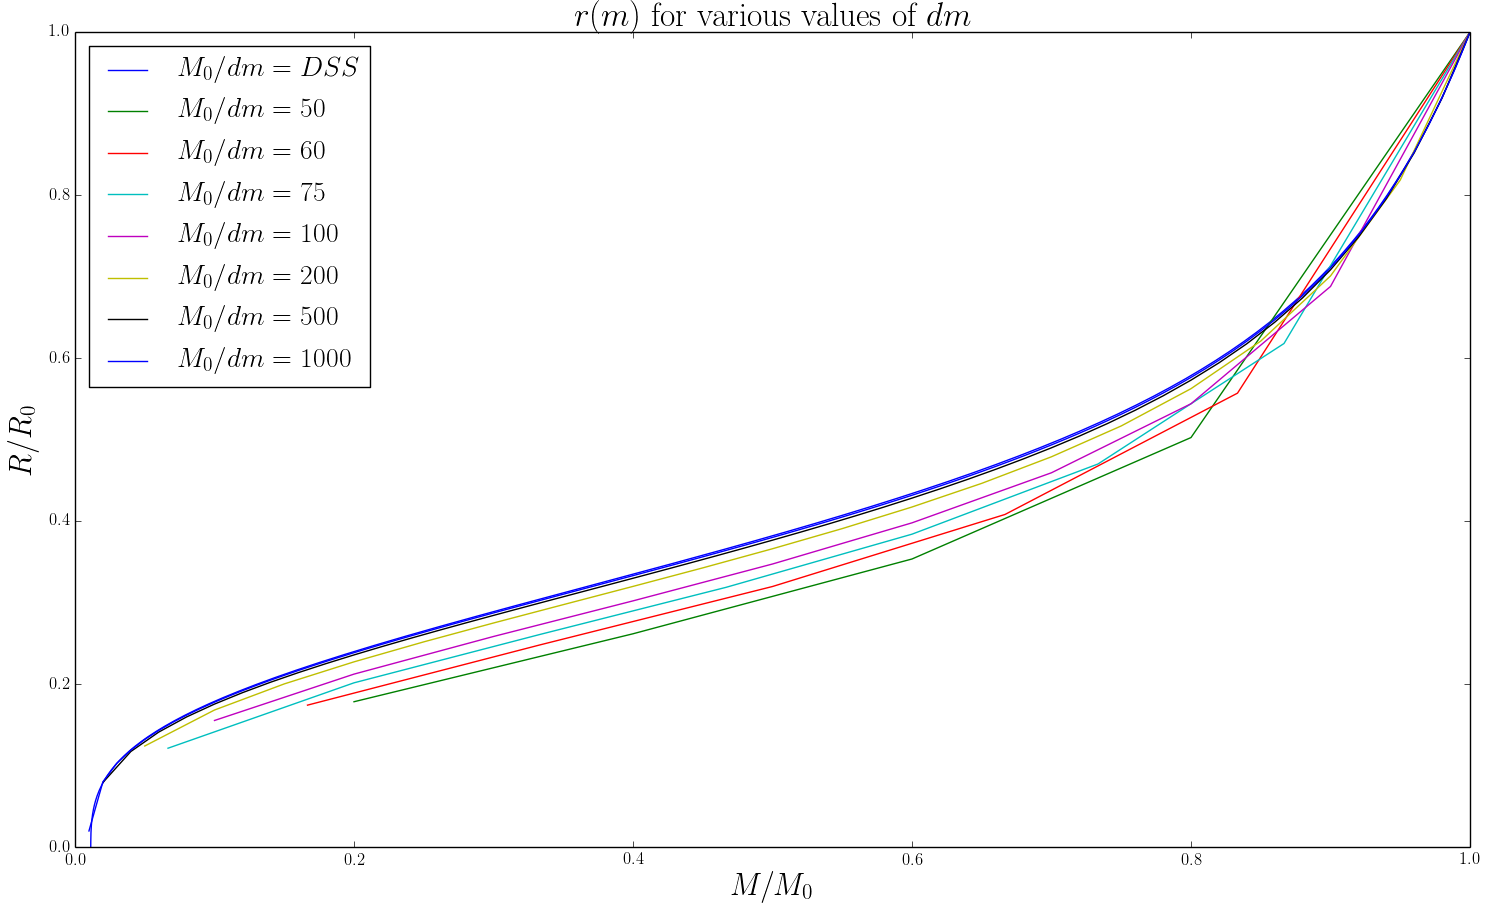
\includegraphics[width=\linewidth]{fig/dm_variation.png}
  \caption{\label{fig:dm_variation} Plots of $r(m)$ using a range of
    different values for $dm$, including the solution obtained when
    using dynamic step size.}
\end{figure*}


\section{Changing the Parameters}
In this numerical model, we have the option to change the initial
parameters to our liking. In particular, we would like to find the set
of initial parameters that give the most realistic model of an actual
star. To this end we are now going to look at how the solution is
affected by changing $R_0,M_0, P_0$ etc. (In the following, $u_{0,i}$
will denote the default initial condition of quantity $u$, as defined
in the exercise text. The defaults correspond to the values for the
Sun at the bottom of the convection layer.)

\subsection{Changing $R_0$}
In order to see the effects of changing the initial radius, figure
\ref{fig:R-variation} has been produced. From the figure we can
conclude with the following for increasing initial radius:

\begin{itemize}
  \item $m$ dies off faster
  \item $P$ becomes \emph{much} smaller
\item $L$ remains constant for much longer (the core becomes a smaller
  fraction of the star)
\item $T$ becomes smaller
\item $\rho$ is similar to $T$, only that $\rho$ becomes \emph{much}
  smaller with increasing $R_0$
\end{itemize}

\begin{figure*}[ht]
  \centering
  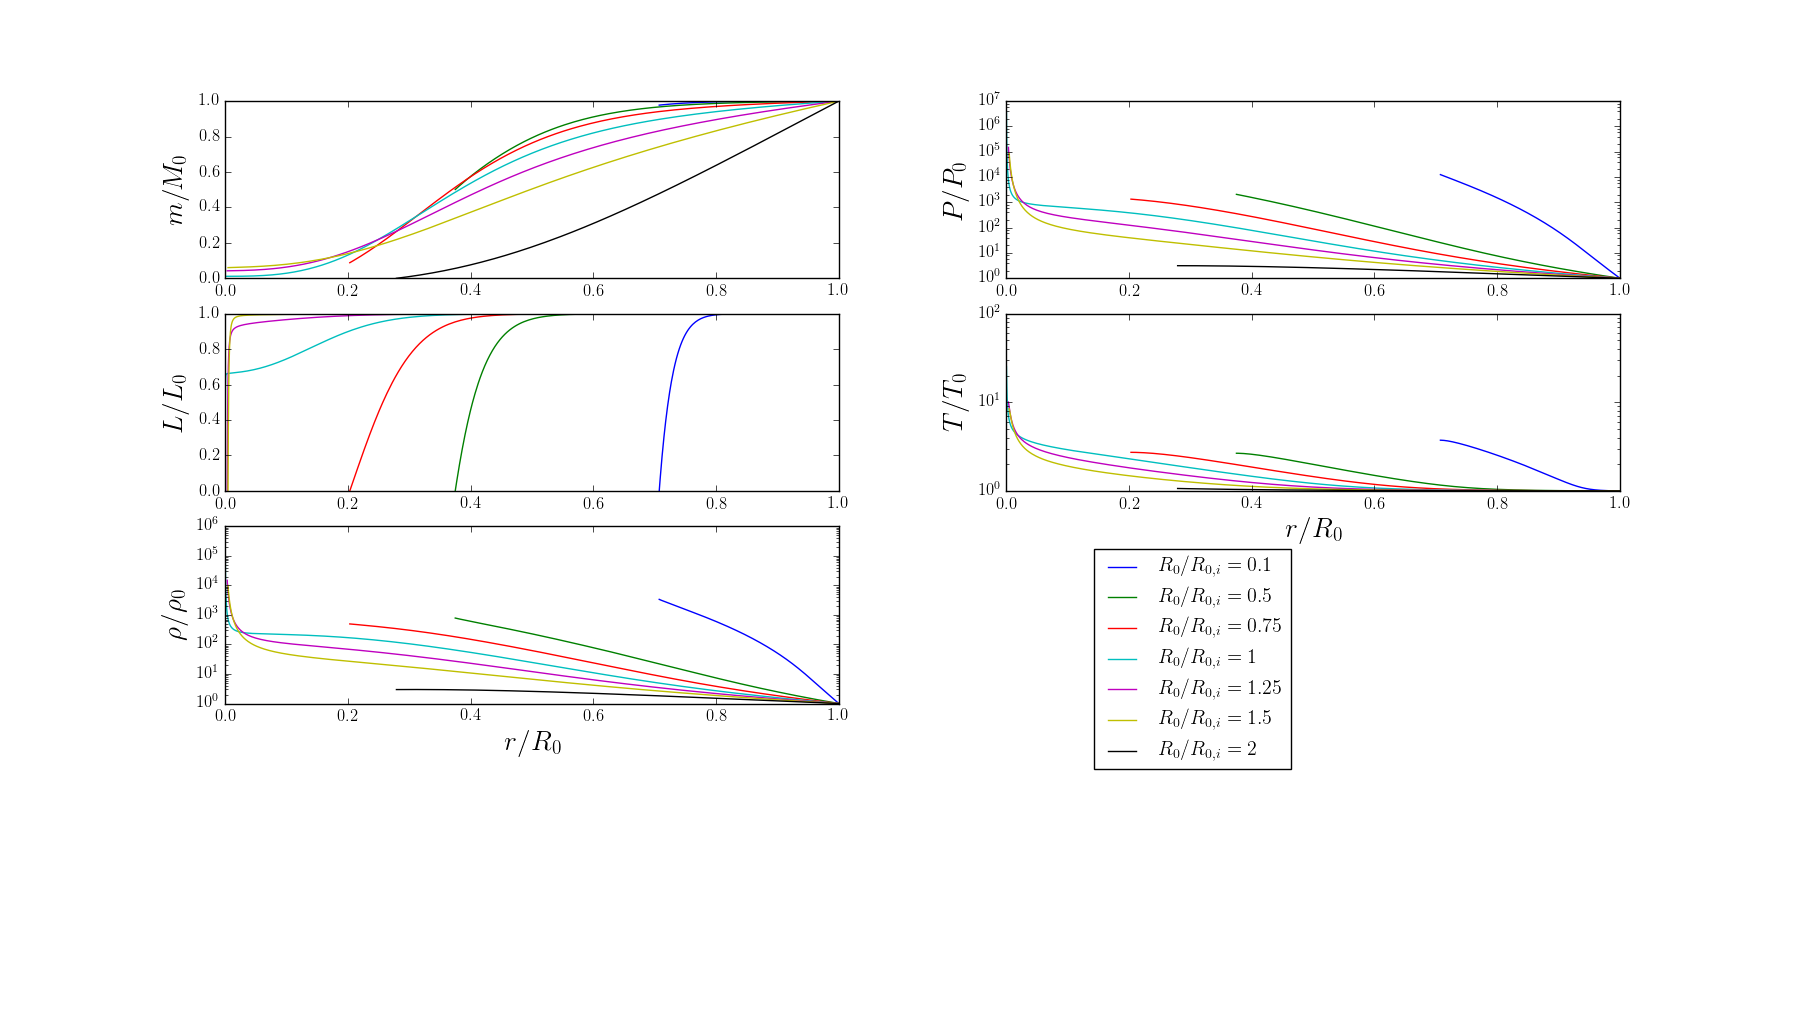
\includegraphics[width=\linewidth]{fig/R_variation.png}
  \caption{\label{fig:R-variation} Plots for all parameters of the star
  showing the effects of changing the initial radius $R_0$.}
\end{figure*}

\subsection{Changing $T_0$}
Figure \ref{fig:T-variation} shows a similar comparison for a change
in the initial temperature $T_0$. We conclude that for increasing
initial temperature we have that:

\begin{itemize}
  \item $m$ falls off less rapidly
  \item $T$ is smaller (relative to $T_0$)
  \item $L$ falls of more rapidly, but at constant radius.
\end{itemize}

The plots for $\rho$ and $P$ are less obvious and does not yield as
clear conclusions. 

\begin{figure*}[ht]
  \centering
  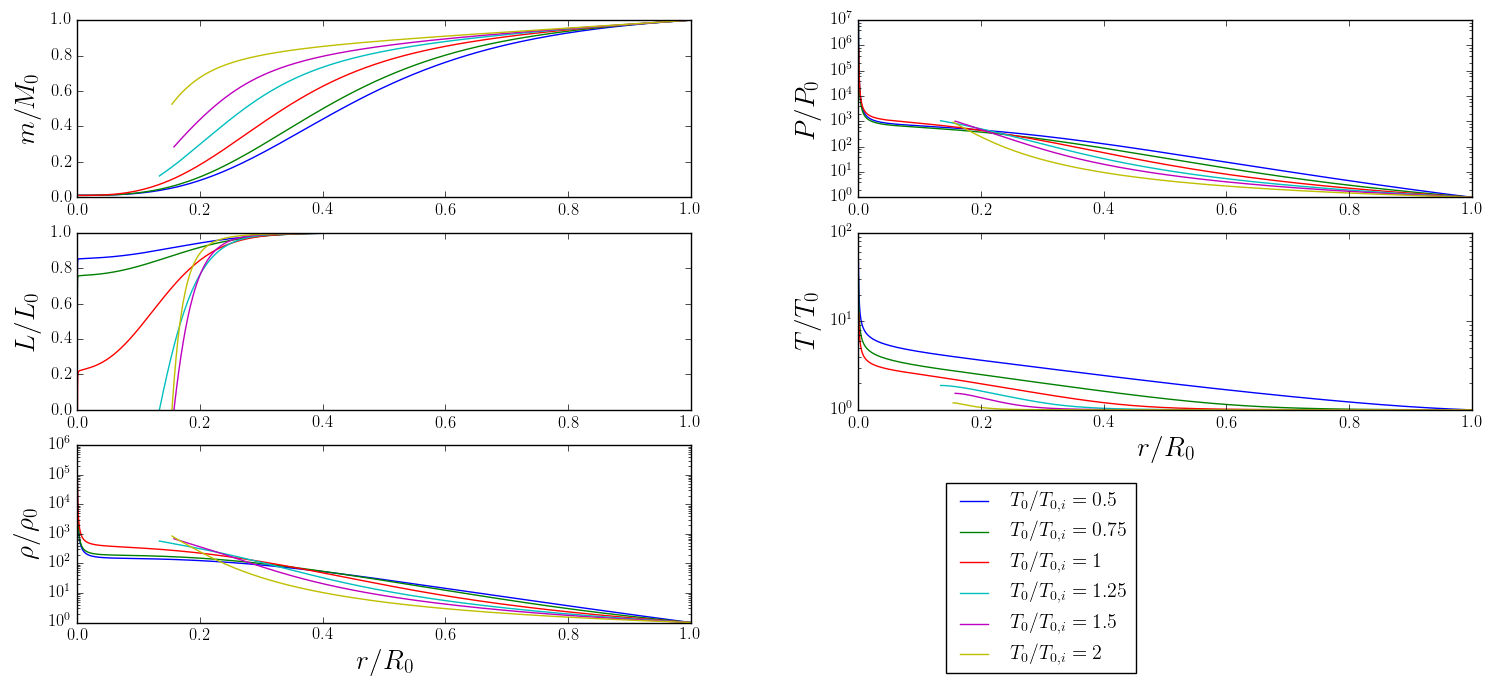
\includegraphics[width=\linewidth]{fig/T_variation.png}
  \caption{\label{fig:T-variation} Plots for all parameters of the star
  showing the effects of changing the initial temperature $T_0$.}
\end{figure*}


\subsection{Changing $\rho_0$}
Figure \ref{fig:rho-variation} shows what happens to the solutions
when we vary the initial density. We conclude that for increasing
initial density we have that:

\begin{itemize}
\item $m$ falls off more rapidly
\item $P$ becomes \emph{much} smaller
\item $\rho$ becomes \emph{much} smaller (exactly in the same way as
  $P$, which is in agreement with Eq. \eqref{eq:rho-eq_state} (linear
  dependence on $P$).)
\end{itemize}

$T$ seems to remain pretty much constant. The plot for $L$ is quite
hard to read due to the higher $\rho_{0}$'s becoming unphysical very
fast. 

\begin{figure*}[ht]
  \centering
  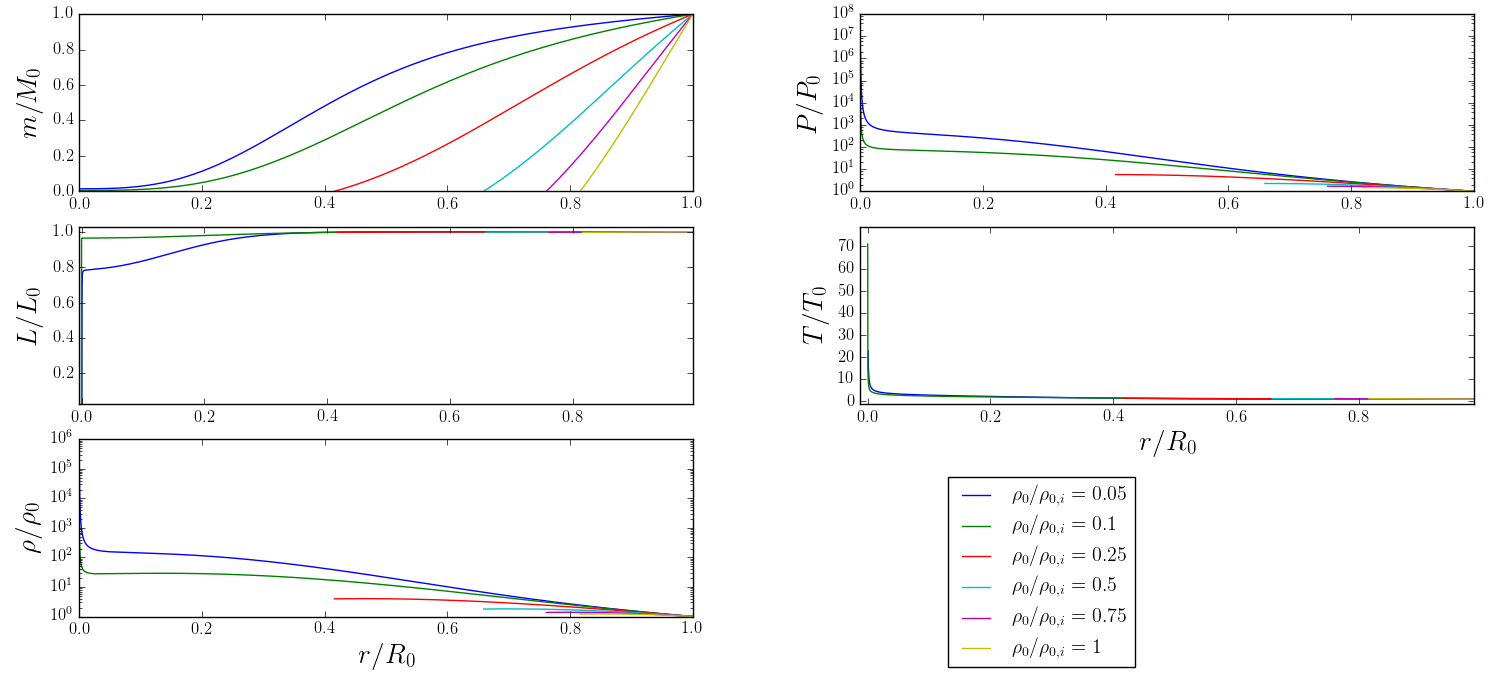
\includegraphics[width=\linewidth]{fig/rho_variation.png}
  \caption{\label{fig:rho-variation} Plots for all parameters of the star
  showing the effects of changing the initial density $\rho_0$.}
\end{figure*}


\subsection{Changing $P_0$}
Figure \ref{fig:P-variation} shows the solutions for a range of
initial pressures. For increasing initial pressure we conclude that:

\begin{itemize}
  \item 
\end{itemize}

\begin{figure}[ht]
  \centering
  \includegraphics[width=\linewidth]{fig/P_variation.png}
  \caption{\label{fig:P-variation} Plots for all parameters of the star
  showing the effects of changing the initial pressure $\P_0$.}
\end{figure}


\onecolumn
\printbibliography
\end{document}

%%% Local Variables:
%%% mode: latex
%%% TeX-master: t
%%% End:
